\documentclass[aspectratio=169,11pt]{beamer}

\usepackage{tikz}
\usetikzlibrary{arrows.meta,positioning,fit,calc,backgrounds}
\usepackage{amsmath,amssymb,booktabs}

% ---------- Colors ----------
\definecolor{maroon}{RGB}{150,45,55}
\definecolor{navy}{RGB}{45,95,150}
\definecolor{lightblue}{RGB}{225,235,245}
\definecolor{lightred}{RGB}{245,230,232}
\definecolor{lightgray}{RGB}{245,245,245}
\definecolor{darkgray}{RGB}{60,60,60}
\definecolor{keepgreen}{RGB}{40,120,80}

\setbeamercolor{structure}{fg=maroon}
\setbeamercolor{block title}{bg=maroon,fg=white}
\setbeamercolor{block body}{bg=lightred,fg=black}
\setbeamercolor{frametitle}{fg=maroon}
\setbeamertemplate{navigation symbols}{}
\setbeamertemplate{footline}[frame number]
\setbeamertemplate{itemize item}{\color{maroon}$\bullet$}

\tikzset{
    op/.style={
        draw=darkgray, rounded corners=2pt, fill=white,
        minimum width=1.55cm, minimum height=0.55cm,
        align=center, font=\scriptsize\bfseries
    },
    plan/.style={
        draw=darkgray, rounded corners=2pt, fill=white,
        minimum width=1.45cm, minimum height=0.52cm,
        align=center, font=\scriptsize
    },
    kept/.style={
        draw=maroon, rounded corners=2pt, fill=lightred,
        minimum width=1.45cm, minimum height=0.52cm,
        align=center, font=\scriptsize\bfseries
    },
    drop/.style={
        draw=gray, rounded corners=2pt, fill=lightgray,
        minimum width=1.45cm, minimum height=0.52cm,
        align=center, font=\scriptsize, text=gray
    },
    box/.style={
        draw=navy, rounded corners=3pt, fill=lightblue,
        inner sep=5pt, align=center, font=\scriptsize
    },
    arr/.style={-{Latex[length=2mm]}, thick, darkgray},
    marr/.style={-{Latex[length=2mm]}, thick, maroon},
    dot/.style={
        circle, draw=darkgray, fill=white,
        inner sep=0pt, minimum size=4.4mm,
        font=\tiny\bfseries, align=center
    },
    dlab/.style={
        draw=none, fill=none, font=\scriptsize\bfseries, maroon, align=center
    }
}

\title{Vector costs and $\alpha$-Pareto pruning\\in Apache Wayang}
\author{Aditya Anand}
\institute{IIT Delhi}
\date{}

\begin{document}

% ============================================================
\begin{frame}{What we implemented}
\begin{columns}[T]
\column{0.50\textwidth}
\begin{block}{The job still runs one plan}
We did not rewrite search.
\texttt{PlanEnumerator} still does
\[
\text{concatenate}\;\to\;\texttt{prune()}
\]
\end{block}
\vspace{0.15cm}
{\small
\begin{itemize}
  \item Cost is now a pair \((c_1,c_2)=(\text{latency},\,\text{money})\).
  \item After each concatenate, keep a Pareto set (or an \(\alpha\)-set).
  \item At the end, pick \(\min c_1\) subject to \(c_2\le B\).
\end{itemize}}
\column{0.48\textwidth}
\centering
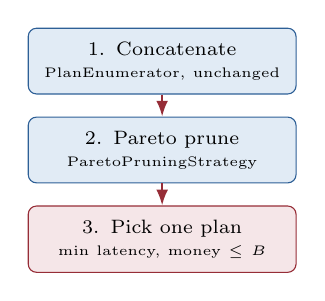
\begin{tikzpicture}[font=\scriptsize]
\node[box, text width=3.05cm] (e) {1. Concatenate\\{\tiny PlanEnumerator, unchanged}};
\node[box, text width=3.05cm, below=0.28cm of e] (p)
    {2. Pareto prune\\{\tiny ParetoPruningStrategy}};
\node[box, text width=3.05cm, below=0.28cm of p, fill=lightred, draw=maroon]
    (k) {3. Pick one plan\\{\tiny min latency, money \(\le B\)}};
\draw[marr] (e) -- (p);
\draw[marr] (p) -- (k);
\end{tikzpicture}

\vspace{0.2cm}
{\scriptsize\color{darkgray}
Money uses Wayang's existing \texttt{TimeToCostConverter}.\\
Java and Spark operators were not rewritten.}
\end{columns}
\end{frame}

% ============================================================
\begin{frame}{1. Enumeration: grow partial plans}

\begin{columns}[c]
\column{0.38\textwidth}
\begin{block}{Wayang already did this}
Walk the operator DAG.
For the next operator, combine every surviving prefix with every mapping of that operator.
\end{block}
\vspace{0.25cm}
{\small
This is \textbf{concatenate}, not a rewrite of join order.

\vspace{0.15cm}
If \(m\) prefixes meet \(n\) mappings, you get up to \(mn\) new candidates. Then prune.}
\column{0.60\textwidth}
\centering
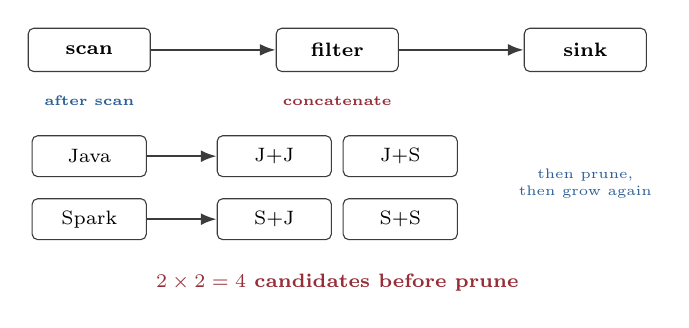
\begin{tikzpicture}[font=\scriptsize]
\node[op] (s) at (0,2.7) {scan};
\node[op] (f) at (3.15,2.7) {filter};
\node[op] (k) at (6.3,2.7) {sink};
\draw[arr] (s) -- (f);
\draw[arr] (f) -- (k);

\node[font=\tiny\bfseries, navy] at (0,2.05) {after scan};
\node[plan] (sj) at (0,1.35) {Java};
\node[plan] (ss) at (0,0.55) {Spark};

\node[font=\tiny\bfseries, maroon] at (3.15,2.05) {concatenate};
\node[plan] (a) at (2.35,1.35) {J$+$J};
\node[plan] (b) at (3.95,1.35) {J$+$S};
\node[plan] (c) at (2.35,0.55) {S$+$J};
\node[plan] (d) at (3.95,0.55) {S$+$S};

\draw[arr] (sj.east) -- (a.west);
\draw[arr] (ss.east) -- (c.west);

\node[font=\tiny, align=center, navy] at (6.3,1.0)
    {then prune,\\then grow again};

\node[font=\scriptsize\bfseries, maroon] at (3.15,-0.25)
    {$2\times 2=4$ candidates before prune};
\end{tikzpicture}
\end{columns}
\end{frame}

% ============================================================
\begin{frame}{2. Only compare plans that can replace each other}

\begin{columns}[c]
\column{0.46\textwidth}
\begin{block}{Same grouping as original Wayang}
Two partial plans compete only if they have
\end{block}
\vspace{0.15cm}
\[
\underbrace{\text{same open operators}}_{\text{the cut}}
\;+\;
\underbrace{\text{same platforms}}_{\text{engines already used}}
\]
\vspace{0.1cm}
{\small
If the open sockets differ, later concatenate cannot swap them, so we must keep both.

\vspace{0.1cm}
This is the old latent-operator grouping. We did not invent a new key.}
\column{0.50\textwidth}
\centering
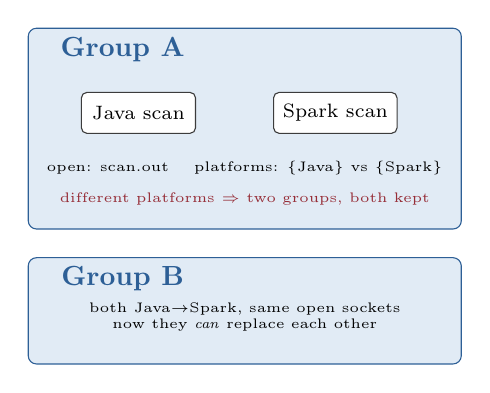
\begin{tikzpicture}[font=\scriptsize]
\node[box, minimum width=5.5cm, minimum height=2.55cm] (g1) at (0,1.05) {};
\node[font=\bfseries, navy] at (-1.55,2.05) {Group A};
\node[plan] at (-1.35,1.25) {Java scan};
\node[plan] at (1.15,1.25) {Spark scan};
\node[font=\tiny] at (0,0.55) {open: scan.out \quad platforms: \{Java\} vs \{Spark\}};
\node[font=\tiny, maroon] at (0,0.15) {different platforms $\Rightarrow$ two groups, both kept};

\node[box, minimum width=5.5cm, minimum height=1.35cm, below=0.35cm of g1] (g2) {};
\node[font=\bfseries, navy] at ($(g2.north)+(-1.55,-0.28)$) {Group B};
\node[font=\tiny, align=center] at ($(g2.center)+(0,-0.08)$)
    {both Java$\to$Spark, same open sockets\\now they \emph{can} replace each other};
\end{tikzpicture}
\end{columns}
\end{frame}

% ============================================================
\begin{frame}{3. Original prune: one scalar winner per group}

\begin{columns}[c]
\column{0.42\textwidth}
\begin{block}{LatentOperatorPruningStrategy}
Inside a group, original Wayang kept the plan with the smallest squashed cost.
\end{block}
\vspace{0.25cm}
{\small
That is lossless \emph{if} cost is one number and additive: a cheaper prefix stays cheaper after concatenate.

\vspace{0.15cm}
It is \textbf{not} lossless for two objectives. The cheaper-but-slower prefix is deleted, so a later hybrid cannot use it.}
\column{0.56\textwidth}
\centering
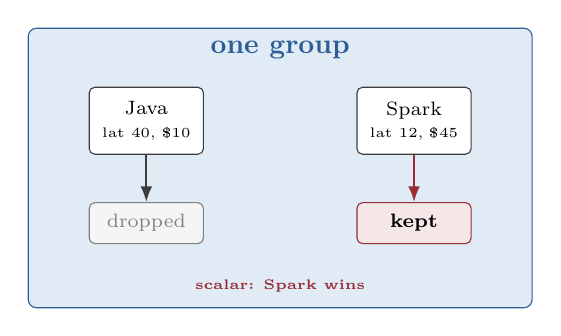
\begin{tikzpicture}[font=\scriptsize]
\node[box, minimum width=6.4cm, minimum height=3.55cm] (g) at (0,0.35) {};
\node[font=\bfseries, navy] at (0,1.85) {one group};

\node[plan, minimum height=0.85cm] (p1) at (-1.7,0.95)
    {Java\\{\tiny lat 40, \$10}};
\node[plan, minimum height=0.85cm] (p2) at (1.7,0.95)
    {Spark\\{\tiny lat 12, \$45}};

\node[drop] (d1) at (-1.7,-0.35) {dropped};
\node[kept] (k2) at (1.7,-0.35) {kept};

\draw[arr] (p1) -- (d1);
\draw[marr] (p2) -- (k2);

\node[font=\tiny\bfseries, maroon] at (0,-1.15)
    {scalar: Spark wins};
\end{tikzpicture}

\vspace{0.1cm}
{\scriptsize\color{maroon} Java is gone. A later cheap join cannot use it.}
\end{columns}
\end{frame}

% ============================================================
\begin{frame}{4. Vector cost: keep the tradeoff}

\begin{columns}[c]
\column{0.46\textwidth}
\begin{block}{What changed}
Enumeration is the same. The cost object is not.
\end{block}
\vspace{0.12cm}
{\small
\texttt{VectorCost} stores
\[
(c_1,\,c_2)=(\text{latency},\,\text{money}).
\]
\(c_1\) from Wayang time estimates.\\
\(c_2\) from \texttt{TimeToCostConverter}
\[
\texttt{fix}+\texttt{per-ms}\times\text{time}.
\]
\vspace{0.08cm}
\(p\) dominates \(q\) if it is \(\le\) on both axes and \(<\) on at least one.

\vspace{0.08cm}
In a group we keep the \textbf{Pareto set}, not one winner.}
\column{0.50\textwidth}
\centering
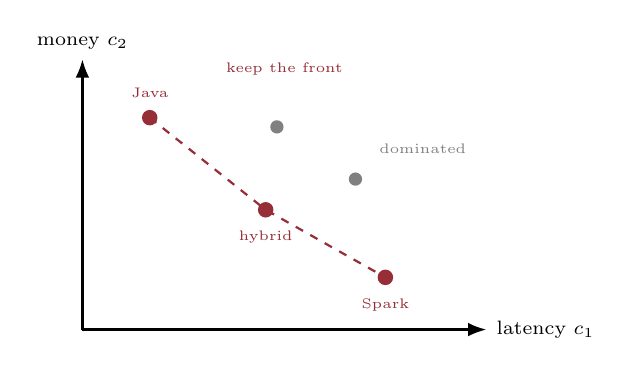
\begin{tikzpicture}[x=0.95cm, y=0.78cm, font=\scriptsize]
\draw[-{Latex}, thick] (0,0) -- (5.4,0) node[right] {latency \(c_1\)};
\draw[-{Latex}, thick] (0,0) -- (0,4.4) node[above] {money \(c_2\)};

\fill[maroon] (0.9,3.45) circle (2.8pt);
\node[maroon, font=\tiny] at (0.9,3.85) {Java};

\fill[maroon] (2.45,1.95) circle (2.8pt);
\node[maroon, font=\tiny] at (2.45,1.50) {hybrid};

\fill[maroon] (4.05,0.85) circle (2.8pt);
\node[maroon, font=\tiny] at (4.05,0.40) {Spark};

\draw[maroon, thick, dashed] (0.9,3.45) -- (2.45,1.95) -- (4.05,0.85);

\fill[gray] (2.6,3.3) circle (2.4pt);
\fill[gray] (3.65,2.45) circle (2.4pt);
\node[gray, font=\tiny] at (4.55,2.95) {dominated};

\node[font=\tiny, maroon] at (2.7,4.25) {keep the front};
\end{tikzpicture}
\end{columns}
\end{frame}

% ============================================================
\begin{frame}{5. Exact Pareto inside a group}

\begin{columns}[c]
\column{0.44\textwidth}
\begin{block}{\texttt{ParetoFront} with \(\varepsilon=0\)}
Two-dimensional staircase:
\begin{enumerate}
  \item sort by latency
  \item scan left to right
  \item keep a plan only if its money is strictly better than the best money so far
\end{enumerate}
\end{block}
\vspace{0.15cm}
{\small
Faster-and-dearer stays. Slower-and-cheaper stays. Worse on both is dropped.}
\column{0.52\textwidth}
\centering
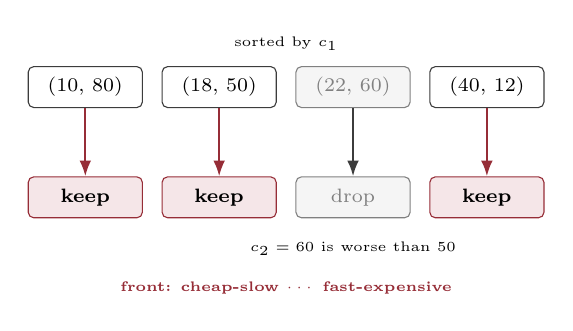
\begin{tikzpicture}[font=\scriptsize]
\node[plan] (a) at (0,2.1) {(10, 80)};
\node[plan] (b) at (1.7,2.1) {(18, 50)};
\node[drop] (c) at (3.4,2.1) {(22, 60)};
\node[plan] (d) at (5.1,2.1) {(40, 12)};

\node[font=\tiny] at (2.55,2.65) {sorted by \(c_1\)};

\node[kept] (ka) at (0,0.7) {keep};
\node[kept] (kb) at (1.7,0.7) {keep};
\node[drop] (kc) at (3.4,0.7) {drop};
\node[kept] (kd) at (5.1,0.7) {keep};

\draw[marr] (a) -- (ka);
\draw[marr] (b) -- (kb);
\draw[arr] (c) -- (kc);
\draw[marr] (d) -- (kd);

\node[font=\tiny] at (3.4,0.05) {\(c_2=60\) is worse than 50};
\node[font=\tiny\bfseries, maroon] at (2.55,-0.45)
    {front: cheap-slow $\cdots$ fast-expensive};
\end{tikzpicture}
\end{columns}
\end{frame}

% ============================================================
\begin{frame}{6. \(\alpha\)-Pareto: shrink a long staircase}

\begin{columns}[T]
\column{0.40\textwidth}
\begin{block}{Why}
An exact front can still be long: many plans, each a little faster and a little dearer.
\end{block}
\vspace{0.12cm}
{\small
Trummer and Koch (SIGMOD 2014): keep an \(\alpha\)-approximate set, \(\alpha=1+\varepsilon\).

\vspace{0.1cm}
Default \(\varepsilon=0.1\), so \(\alpha=1.1\).

\vspace{0.12cm}
Plan \(a\) \(\alpha\)-dominates \(b\) if
\[
a_i \le \alpha\, b_i \quad \forall i.
\]
Every discarded plan has a kept plan that is at most \(\alpha\) worse on both axes.}
\column{0.58\textwidth}
\centering
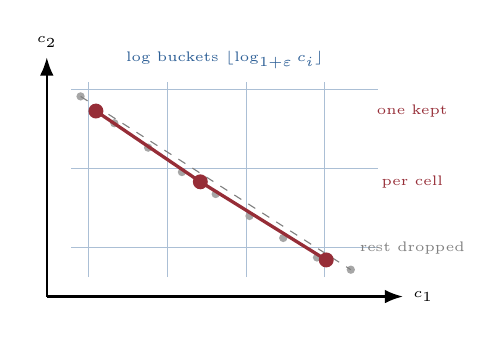
\begin{tikzpicture}[x=0.78cm, y=0.62cm, font=\tiny]
% grid of log buckets
\draw[navy!40, thin] (1,1) grid (6,5);
\node[navy] at (3.5,5.45) {log buckets \(\lfloor\log_{1+\varepsilon} c_i\rfloor\)};

% many exact-front points
\foreach \x/\y in {1.15/4.7, 1.7/4.15, 2.25/3.65, 2.8/3.15, 3.35/2.7, 3.9/2.25, 4.45/1.8, 5.0/1.4, 5.55/1.15} {
  \fill[gray!70] (\x,\y) circle (1.5pt);
}
\draw[gray, dashed] (1.15,4.7) -- (5.55,1.15);

% kept representatives
\fill[maroon] (1.4,4.4) circle (2.7pt);
\fill[maroon] (3.1,2.95) circle (2.7pt);
\fill[maroon] (5.15,1.35) circle (2.7pt);
\draw[maroon, very thick] (1.4,4.4) -- (3.1,2.95) -- (5.15,1.35);

\node[maroon] at (6.55,4.4) {one kept};
\node[maroon] at (6.55,2.95) {per cell};
\node[gray] at (6.55,1.6) {rest dropped};

\draw[-{Latex}, thick] (0.6,0.6) -- (6.4,0.6) node[right] {\(c_1\)};
\draw[-{Latex}, thick] (0.6,0.6) -- (0.6,5.5) node[above] {\(c_2\)};
\end{tikzpicture}

\vspace{0.05cm}
{\scriptsize Same cell \(\Rightarrow\) costs differ by at most factor \(\alpha\). Keep one, then run exact Pareto on those.}
\end{columns}
\end{frame}

% ============================================================
\begin{frame}{7. One dimensional log buckets}

\begin{columns}[T]
\column{0.42\textwidth}
\vspace{0.08cm}
{\small
One cost \(c>0\), \(\varepsilon>0\):
\[
b(c)=\bigl\lfloor \ln c \big/ \ln(1+\varepsilon) \bigr\rfloor
\]
Bucket \(k\) is
\[
\bigl[(1+\varepsilon)^k,\,(1+\varepsilon)^{k+1}\bigr).
\]

\vspace{0.12cm}
Same bucket \(\Rightarrow\) the two costs differ by at most factor \(\alpha=1+\varepsilon\).

\vspace{0.12cm}
Keep \textbf{one} plan in that interval.

\vspace{0.12cm}
{\scriptsize Picture uses \(\varepsilon=1\) (easy cuts). Code default is \(\varepsilon=0.1\).}}
\column{0.56\textwidth}
\centering
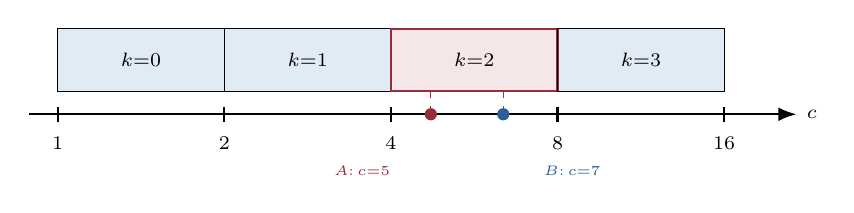
\begin{tikzpicture}[font=\scriptsize, >=Latex, scale=0.92]
\draw[-{Latex}, thick] (0,0) -- (10.6,0) node[right] {\(c\)};
\foreach \x/\lab in {0.4/1, 2.7/2, 5.0/4, 7.3/8, 9.6/16} {
  \draw[thick] (\x,0.1) -- (\x,-0.1);
  \node[below] at (\x,-0.18) {\lab};
}
\fill[lightblue] (0.4,0.32) rectangle (2.7,1.18);
\fill[lightblue] (2.7,0.32) rectangle (5.0,1.18);
\fill[lightred] (5.0,0.32) rectangle (7.3,1.18);
\fill[lightblue] (7.3,0.32) rectangle (9.6,1.18);
\draw (0.4,0.32) rectangle (2.7,1.18);
\draw (2.7,0.32) rectangle (5.0,1.18);
\draw[maroon, thick] (5.0,0.32) rectangle (7.3,1.18);
\draw (7.3,0.32) rectangle (9.6,1.18);
\node at (1.55,0.75) {\(k{=}0\)};
\node at (3.85,0.75) {\(k{=}1\)};
\node at (6.15,0.75) {\(k{=}2\)};
\node at (8.45,0.75) {\(k{=}3\)};
\fill[maroon] (5.55,0) circle (2.4pt);
\fill[navy] (6.55,0) circle (2.4pt);
\draw[maroon, dashed] (5.55,0) -- (5.55,0.32);
\draw[navy, dashed] (6.55,0) -- (6.55,0.32);
\node[maroon, below=0.42cm, align=center, font=\tiny] at (4.6,-0.12) {\(A{:}\,c{=}5\)};
\node[navy, below=0.42cm, align=center, font=\tiny] at (7.5,-0.12) {\(B{:}\,c{=}7\)};
\end{tikzpicture}

\vspace{0.35cm}
{\scriptsize \(A\) and \(B\) both in \([4,8)\). Merge them. \(c{=}9\) would be \(k{=}3\), a different cell.

\vspace{0.08cm}
Adjacent buckets can still split two values that are within \(\alpha\). Same cell is sufficient, not necessary.}
\end{columns}
\end{frame}

% ============================================================
\begin{frame}{8. Two dimensions: the pair of buckets}

\vspace{0.06cm}
\centering
{\small No extra 2-D formula. Call the same \(b(\cdot)\) on latency and on money. The cell is \((b(c_1),\,b(c_2))\).}

\vspace{0.18cm}
\begin{columns}[T]
\column{0.58\textwidth}
\centering
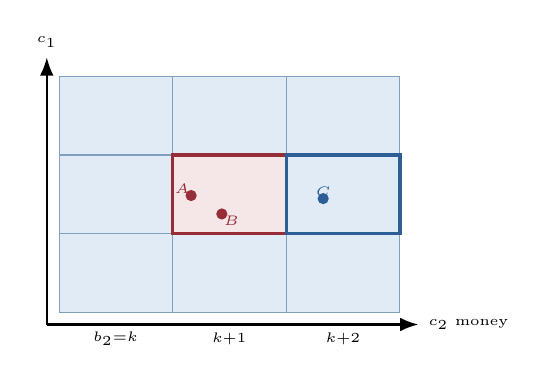
\begin{tikzpicture}[font=\tiny, scale=0.78]
\def\W{1.85}
\def\H{1.28}
\foreach \i in {0,1,2} {
  \foreach \j in {0,1,2} {
    \fill[lightblue] ({0.55+\i*\W},{0.55+\j*\H}) rectangle ({0.55+(\i+1)*\W},{0.55+(\j+1)*\H});
    \draw[navy!60] ({0.55+\i*\W},{0.55+\j*\H}) rectangle ({0.55+(\i+1)*\W},{0.55+(\j+1)*\H});
  }
}
\fill[lightred] ({0.55+1*\W},{0.55+1*\H}) rectangle ({0.55+2*\W},{0.55+2*\H});
\draw[maroon, very thick] ({0.55+1*\W},{0.55+1*\H}) rectangle ({0.55+2*\W},{0.55+2*\H});
\draw[navy, very thick] ({0.55+2*\W},{0.55+1*\H}) rectangle ({0.55+3*\W},{0.55+2*\H});
\fill[maroon] (2.7,2.45) circle (2.6pt);
\node[maroon, above left, inner sep=0.5pt] at (2.7,2.45) {\(A\)};
\fill[maroon] (3.2,2.15) circle (2.6pt);
\node[maroon, below right, inner sep=0.5pt] at (3.2,2.15) {\(B\)};
\fill[navy] (4.85,2.4) circle (2.6pt);
\node[navy, above, inner sep=0.5pt] at (4.85,2.4) {\(C\)};
\draw[-{Latex}, thick] (0.35,0.35) -- (6.4,0.35) node[right] {\(c_2\) money};
\draw[-{Latex}, thick] (0.35,0.35) -- (0.35,4.7) node[above] {\(c_1\)};
\node at (1.47,0.12) {\(b_2{=}k\)};
\node at (3.32,0.12) {\(k{+}1\)};
\node at (5.17,0.12) {\(k{+}2\)};
\end{tikzpicture}
\column{0.40\textwidth}
\vspace{0.25cm}
{\small
\textbf{Red cell.} \(A\) and \(B\) share both indices. Mutually \(\alpha\)-dominate. Keep one.

\vspace{0.28cm}
\textbf{Blue outline.} \(C\) shares the latency bucket, not the money bucket. Different map key. Not merged.

\vspace{0.28cm}
\texttt{logBuckets} returns two longs.\\
\texttt{Map} key \(= (b_1,b_2)\).

\vspace{0.2cm}
{\scriptsize At most \(N^2\) cells if each axis has \(N\) buckets. Then exact Pareto leaves about \(N\).}}
\end{columns}
\end{frame}

% ============================================================
\begin{frame}{9. Example in the code (\(\varepsilon=0.1\))}

\centering
\renewcommand{\arraystretch}{1.18}
\setlength{\tabcolsep}{8pt}
{\small
\begin{tabular}{@{}lrrrrl@{}}
\toprule
plan & \(c_1\) & \(c_2\) & \(b(c_1)\) & \(b(c_2)\) & cell \\
\midrule
\(A\) & 100 & 50 & 48 & 41 & \((48,41)\) \\
\(B\) & 105 & 52 & 48 & 41 & same as \(A\) \\
\(C\) & 100 & 80 & 48 & 45 & \((48,45)\) \\
\bottomrule
\end{tabular}}

\vspace{0.32cm}
\begin{columns}[T]
\column{0.46\textwidth}
{\small
\(A\) and \(B\) collide. Keep \(A\) (faster, then cheaper).

\vspace{0.18cm}
\(C\) is another cell. Exact Pareto then drops \(C\) (no faster, more money).

\vspace{0.22cm}
{\scriptsize This runs after \textbf{every} concatenate, on that group's list. Not once at the end. IRA is not implemented.}}
\column{0.50\textwidth}
\centering
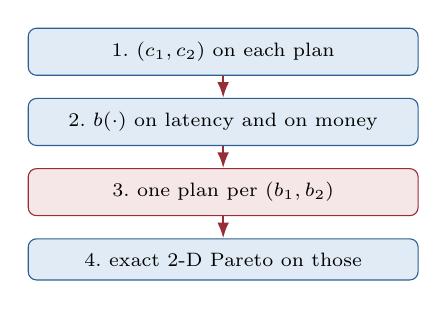
\begin{tikzpicture}[font=\scriptsize, node distance=0.30cm]
\node[box, text width=4.6cm] (a) {1.\ \((c_1,c_2)\) on each plan};
\node[box, text width=4.6cm, below=0.28cm of a] (b) {2.\ \(b(\cdot)\) on latency and on money};
\node[box, text width=4.6cm, fill=lightred, draw=maroon, below=0.28cm of b] (c) {3.\ one plan per \((b_1,b_2)\)};
\node[box, text width=4.6cm, below=0.28cm of c] (d) {4.\ exact 2-D Pareto on those};
\draw[marr] (a) -- (b);
\draw[marr] (b) -- (c);
\draw[marr] (c) -- (d);
\end{tikzpicture}
\end{columns}
\end{frame}

% ============================================================
\begin{frame}{10. What the prune code actually does}

\centering
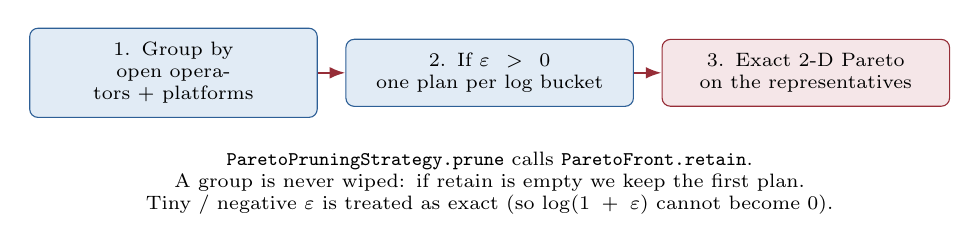
\begin{tikzpicture}[font=\small, node distance=0.42cm]
\node[box, text width=3.3cm] (g) {1. Group by\\open operators $+$ platforms};
\node[box, text width=3.3cm, right=0.35cm of g] (b)
    {2. If \(\varepsilon>0\)\\one plan per log bucket};
\node[box, text width=3.3cm, right=0.35cm of b, fill=lightred, draw=maroon]
    (p) {3. Exact 2-D Pareto\\on the representatives};

\draw[marr] (g) -- (b);
\draw[marr] (b) -- (p);

\node[font=\scriptsize, below=0.45cm of b, text width=11.5cm, align=center] {
\texttt{ParetoPruningStrategy.prune} calls \texttt{ParetoFront.retain}.\\
A group is never wiped: if retain is empty we keep the first plan.\\
Tiny / negative \(\varepsilon\) is treated as exact (so \(\log(1+\varepsilon)\) cannot become 0).};
\end{tikzpicture}

\vspace{0.55cm}
\begin{columns}[T]
\column{0.48\textwidth}
{\scriptsize\bfseries Default properties}\\[0.15cm]
{\ttfamily\scriptsize
pruning = ParetoPruningStrategy\\
cost.model = vector\\
epsilon = 0.1\\
weight.latency = 1\\
weight.monetary = 0}
\column{0.50\textwidth}
{\scriptsize\bfseries Additive costs}\\[0.15cm]
{\scriptsize
Concatenate \emph{sums} the two vectors.\\
A dominated prefix cannot become undominated later, so prune-after-concat is safe.}
\end{columns}
\end{frame}

% ============================================================
\begin{frame}{11. Final pick: one plan, not the whole front}

\begin{columns}[c]
\column{0.46\textwidth}
\begin{block}{\texttt{VectorPlanSelection.pick}}
Among complete plans with \(c_2\le B\), take the smallest \(c_1\).
\end{block}
\vspace{0.12cm}
{\small
\begin{itemize}
  \item If none fit \(B\), take cheapest money.
  \item Default weights \((1,0)\): fastest under the budget.
  \item \(B\) is applied \textbf{only at the end}, not on each operator.
\end{itemize}
\vspace{0.08cm}
\texttt{selectBest} is the paper weighted sum. The live optimizer uses \texttt{pick}.}
\column{0.50\textwidth}
\centering
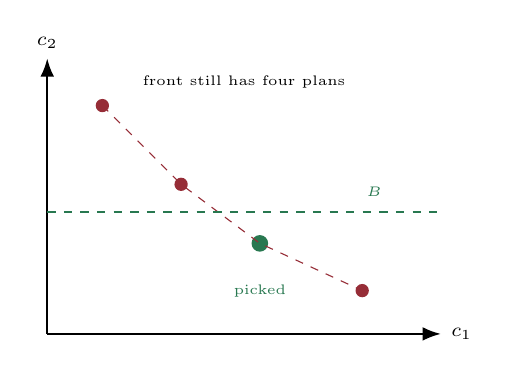
\begin{tikzpicture}[font=\scriptsize]
\draw[-{Latex}, thick] (0,0) -- (5.0,0) node[right] {\(c_1\)};
\draw[-{Latex}, thick] (0,0) -- (0,3.5) node[above] {\(c_2\)};
\fill[maroon] (0.7,2.9) circle (2.4pt);
\fill[maroon] (1.7,1.9) circle (2.4pt);
\fill[keepgreen] (2.7,1.15) circle (3pt);
\fill[maroon] (4.0,0.55) circle (2.4pt);
\draw[maroon, dashed] (0.7,2.9) -- (1.7,1.9) -- (2.7,1.15) -- (4.0,0.55);
\draw[keepgreen, thick, dashed] (0,1.55) -- (5.0,1.55);
\node[keepgreen, font=\tiny] at (4.15,1.8) {\(B\)};
\node[keepgreen, font=\tiny] at (2.7,0.55) {picked};
\node[font=\tiny] at (2.5,3.2) {front still has four plans};
\end{tikzpicture}
\end{columns}
\end{frame}

% ============================================================
\begin{frame}{12. Walk-through: why a hybrid survives}

\centering
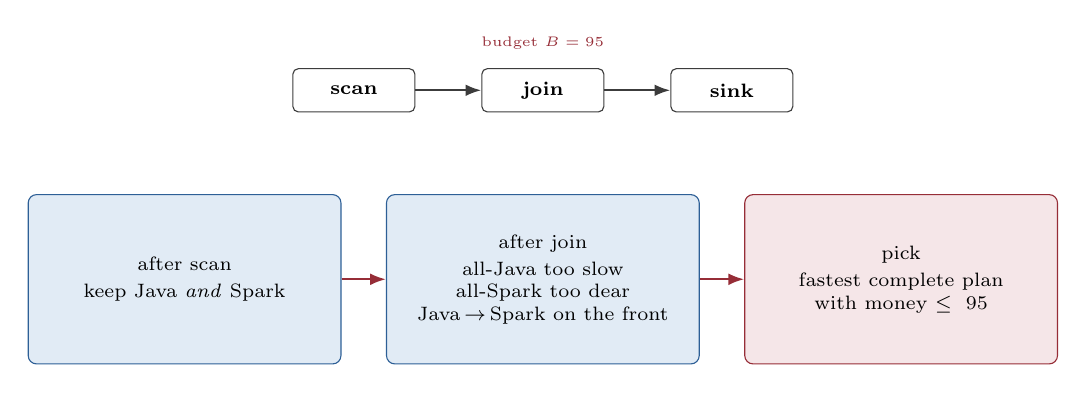
\begin{tikzpicture}[font=\scriptsize]
\node[op] (s) at (-2.4,2.55) {scan};
\node[op] (j) at (0,2.55) {join};
\node[op] (k) at (2.4,2.55) {sink};
\draw[arr] (s) -- (j);
\draw[arr] (j) -- (k);
\node[font=\tiny, maroon] at (0,3.15) {budget \(B=95\)};

\node[box, text width=3.55cm, minimum height=2.15cm, inner sep=6pt]
    (a) at (-4.55,0.15) {after scan\\[2pt]keep Java \emph{and} Spark};
\node[box, text width=3.55cm, minimum height=2.15cm, inner sep=6pt]
    (b) at (0,0.15) {after join\\[2pt]all-Java too slow\\all-Spark too dear\\Java$\,\to\,$Spark on the front};
\node[box, text width=3.55cm, minimum height=2.15cm, inner sep=6pt,
      fill=lightred, draw=maroon]
    (c) at (4.55,0.15) {pick\\[2pt]fastest complete plan\\with money \(\le 95\)};

\draw[marr] (a) -- (b);
\draw[marr] (b) -- (c);
\end{tikzpicture}

\vspace{0.35cm}
\begin{columns}[T]
\column{0.46\textwidth}
{\small\textbf{Original Wayang}\\[0.2cm]
Scalar prune often keeps only Spark after scan. The hybrid prefix is already gone.}
\column{0.46\textwidth}
{\small\textbf{Now}\\[0.2cm]
Both prefixes stay until the pick. The five-engine simulation matches exhaustive search on that hybrid.}
\end{columns}
\end{frame}

% ============================================================
\begin{frame}{13. Code we added and code we only hooked}

{\small
\begin{tabular}{@{}lll@{}}
\toprule
 & \textbf{Class} & \textbf{Role} \\
\midrule
New & \texttt{VectorCost} & pair, dominance, \(\alpha\)-dominance, log buckets \\
New & \texttt{VectorEstimatableCost} & fill \((c_1,c_2)\), call the pick \\
New & \texttt{ParetoFront} & exact staircase, then RTA buckets \\
New & \texttt{ParetoPruningStrategy} & default \texttt{prune()} after concatenate \\
New & \texttt{VectorPlanSelection} & \(\min c_1\) s.t.\ \(c_2\le B\) \\
\midrule
Edited & \texttt{EstimatableCost} & default vector method so old models compile \\
Edited & \texttt{PlanImplementation} & \texttt{getVectorCostEstimate()} \\
Edited & \texttt{LatentOperatorPruningStrategy} & optional Pareto if vector flag is on \\
Edited & \texttt{Configuration} & \texttt{cost.model=vector} \\
Edited & \texttt{wayang-core-defaults.properties} & \(\varepsilon\), weights, optional \(B\) \\
\bottomrule
\end{tabular}}

\vspace{0.35cm}
{\small
\texttt{PlanEnumerator.java} is original. Channel conversion is still one scalar path.
IRA (tighten \(\varepsilon\) until a hard bound is proven) is not implemented.}
\end{frame}

% ============================================================
\begin{frame}{14. How we tested}

\centering
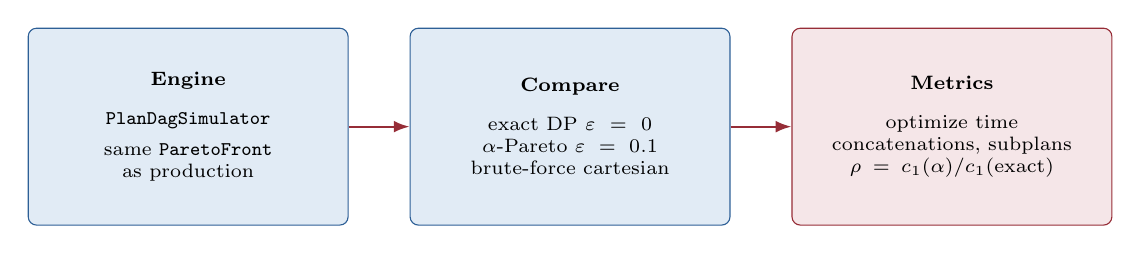
\begin{tikzpicture}[font=\small]
\node[box, text width=3.5cm, minimum height=2.5cm, inner sep=8pt] (a) at (-4.85,0.35)
    {\textbf{Engine}\\[6pt]
    \texttt{PlanDagSimulator}\\[3pt]
    same \texttt{ParetoFront}\\
    as production};
\node[box, text width=3.5cm, minimum height=2.5cm, inner sep=8pt] (b) at (0,0.35)
    {\textbf{Compare}\\[6pt]
    exact DP \(\varepsilon=0\)\\
    $\alpha$-Pareto \(\varepsilon=0.1\)\\
    brute-force cartesian};
\node[box, text width=3.5cm, minimum height=2.5cm, inner sep=8pt, fill=lightred, draw=maroon] (c) at (4.85,0.35)
    {\textbf{Metrics}\\[6pt]
    optimize time\\
    concatenations, subplans\\
    \(\rho=c_1(\alpha)/c_1(\mathrm{exact})\)};
\draw[marr] (a) -- (b);
\draw[marr] (b) -- (c);
\end{tikzpicture}

\vspace{0.45cm}
{\small
Synthetic \((c_1,c_2)\) vectors, additive costs. Not a live Spark job.\\[4pt]
A budget miss (exact fits \(B\), \(\alpha\) does not) is counted as \(\rho=+\infty\).}
\end{frame}

% ============================================================
\begin{frame}{15. DAG shapes we built}

\centering
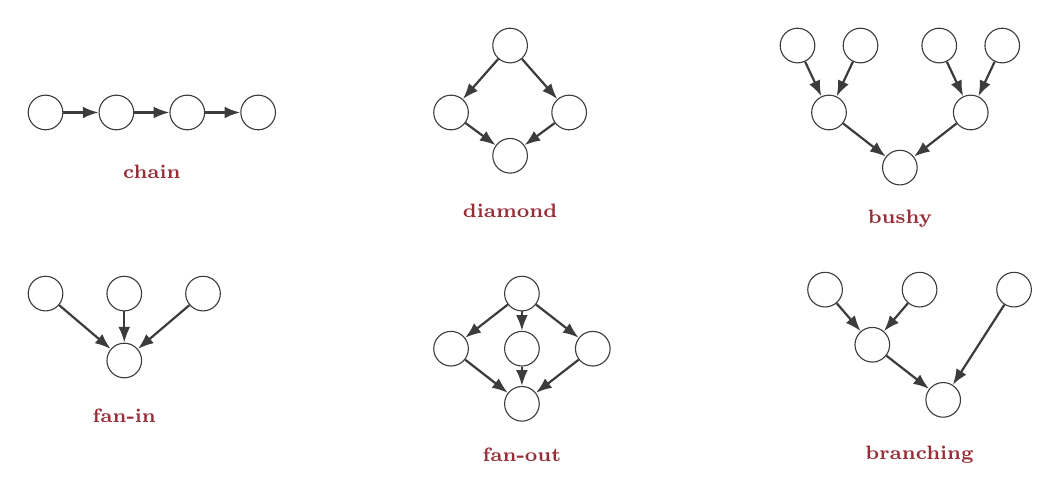
\begin{tikzpicture}
% ----- chain -----
\begin{scope}[shift={(-5.0,1.85)}]
  \node[dot] (a) at (0,0) {};
  \node[dot] (b) at (0.9,0) {};
  \node[dot] (c) at (1.8,0) {};
  \node[dot] (d) at (2.7,0) {};
  \draw[arr] (a) -- (b);
  \draw[arr] (b) -- (c);
  \draw[arr] (c) -- (d);
  \node[dlab] at (1.35,-0.75) {chain};
\end{scope}

% ----- diamond -----
\begin{scope}[shift={(0.0,1.85)}]
  \node[dot] (s) at (0.9,0.85) {};
  \node[dot] (l) at (0.15,0) {};
  \node[dot] (r) at (1.65,0) {};
  \node[dot] (j) at (0.9,-0.55) {};
  \draw[arr] (s) -- (l);
  \draw[arr] (s) -- (r);
  \draw[arr] (l) -- (j);
  \draw[arr] (r) -- (j);
  \node[dlab] at (0.9,-1.25) {diamond};
\end{scope}

% ----- bushy -----
\begin{scope}[shift={(4.55,1.85)}]
  \node[dot] (s1) at (0,0.85) {};
  \node[dot] (s2) at (0.8,0.85) {};
  \node[dot] (s3) at (1.8,0.85) {};
  \node[dot] (s4) at (2.6,0.85) {};
  \node[dot] (j1) at (0.4,0) {};
  \node[dot] (j2) at (2.2,0) {};
  \node[dot] (j3) at (1.3,-0.7) {};
  \draw[arr] (s1) -- (j1);
  \draw[arr] (s2) -- (j1);
  \draw[arr] (s3) -- (j2);
  \draw[arr] (s4) -- (j2);
  \draw[arr] (j1) -- (j3);
  \draw[arr] (j2) -- (j3);
  \node[dlab] at (1.3,-1.35) {bushy};
\end{scope}

% ----- fan-in -----
\begin{scope}[shift={(-5.0,-1.15)}]
  \node[dot] (f1) at (0,0.7) {};
  \node[dot] (f2) at (1.0,0.7) {};
  \node[dot] (f3) at (2.0,0.7) {};
  \node[dot] (fj) at (1.0,-0.15) {};
  \draw[arr] (f1) -- (fj);
  \draw[arr] (f2) -- (fj);
  \draw[arr] (f3) -- (fj);
  \node[dlab] at (1.0,-0.85) {fan-in};
\end{scope}

% ----- fan-out -----
\begin{scope}[shift={(0.15,-1.15)}]
  \node[dot] (o) at (0.9,0.7) {};
  \node[dot] (o1) at (0,0) {};
  \node[dot] (o2) at (0.9,0) {};
  \node[dot] (o3) at (1.8,0) {};
  \node[dot] (oj) at (0.9,-0.7) {};
  \draw[arr] (o) -- (o1);
  \draw[arr] (o) -- (o2);
  \draw[arr] (o) -- (o3);
  \draw[arr] (o1) -- (oj);
  \draw[arr] (o2) -- (oj);
  \draw[arr] (o3) -- (oj);
  \node[dlab] at (0.9,-1.35) {fan-out};
\end{scope}

% ----- branch -----
\begin{scope}[shift={(4.7,-1.15)}]
  \node[dot] (b1) at (0.2,0.75) {};
  \node[dot] (b2) at (1.4,0.75) {};
  \node[dot] (b3) at (2.6,0.75) {};
  \node[dot] (bj1) at (0.8,0.05) {};
  \node[dot] (bj2) at (1.7,-0.65) {};
  \draw[arr] (b1) -- (bj1);
  \draw[arr] (b2) -- (bj1);
  \draw[arr] (bj1) -- (bj2);
  \draw[arr] (b3) -- (bj2);
  \node[dlab] at (1.4,-1.35) {branching};
\end{scope}
\end{tikzpicture}

\vspace{0.15cm}
{\small Also two- and three-diamonds, left-deep joins, skip edges, and 40 random connected DAGs.}
\end{frame}

% ============================================================
\begin{frame}{16. Exact DP matches brute force}

\begin{columns}[T]
\column{0.48\textwidth}
\vspace{0.15cm}
\begin{block}{35 small graphs}
Every budget pick of exact Pareto DP (\(\varepsilon=0\)) matched exhaustive cartesian search.
\end{block}
\vspace{0.35cm}
{\small
Chains 3--6 ops, diamonds, bushy, fan-in/out, skip edges, left-deep, and 12 random DAGs.

\vspace{0.2cm}
Budgets at 10\%, 40\%, 80\% of the money range, plus unconstrained.}
\column{0.48\textwidth}
\vspace{0.15cm}
\centering
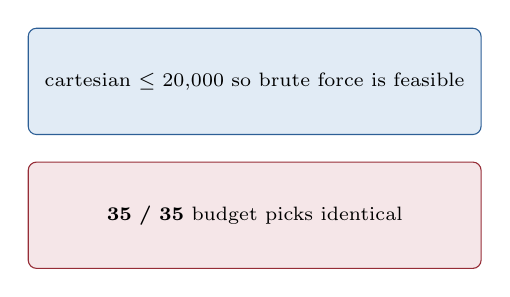
\begin{tikzpicture}[font=\small]
\node[box, text width=5.4cm, minimum height=1.35cm] at (0,1.35)
    {cartesian $\le 20{,}000$ so brute force is feasible};
\node[box, text width=5.4cm, minimum height=1.35cm, fill=lightred, draw=maroon] at (0,-0.35)
    {\textbf{35 / 35} budget picks identical};
\end{tikzpicture}
\end{columns}
\end{frame}

% ============================================================
\begin{frame}{17. Speed vs quality on a long chain}

\vspace{0.1cm}
\centering
{\small 12 operators, 12 platforms. Cartesian size about \(10^{12}\).}

\vspace{0.35cm}
\renewcommand{\arraystretch}{1.28}
\setlength{\tabcolsep}{10pt}
{\small
\begin{tabular}{@{}lcccc@{}}
\toprule
\(\varepsilon\) & concatenations & subplans & time & \(\rho\) \\
\midrule
0 (exact) & 103k & 134 & 24\,ms & 1.00 \\
\textbf{0.1 (default)} & \textbf{20k} & \textbf{21} & \textbf{6\,ms} & \textbf{1.00} \\
0.25 & 10k & 11 & 2\,ms & 1.06 \\
0.5 & 6k & 5 & 1.4\,ms & 1.28 \\
1.0 & 4k & 3 & 1.1\,ms & 1.18 \\
\bottomrule
\end{tabular}}

\vspace{0.45cm}
{\small
Default \(\varepsilon=0.1\) kept the \textbf{same pick} as exact, with about 80\% fewer concatenations.\\[4pt]
Bigger \(\varepsilon\): fewer subplans, faster search, a slightly worse pick.}
\end{frame}

% ============================================================
\begin{frame}{18. Shape $\times$ size: 65 graphs}

\centering
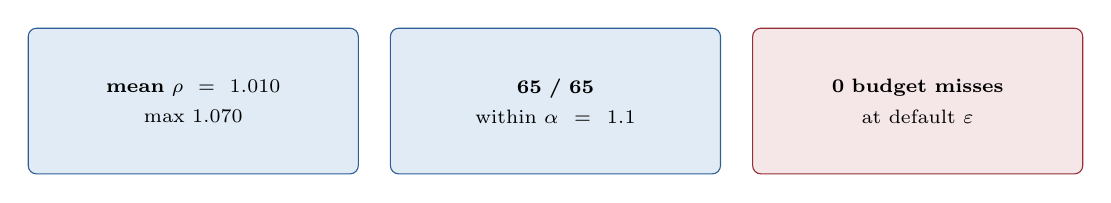
\begin{tikzpicture}[font=\small]
\node[box, text width=3.7cm, minimum height=1.85cm, inner sep=7pt] at (-4.6,0.9)
    {\textbf{mean \(\rho=1.010\)}\\[3pt]max \(1.070\)};
\node[box, text width=3.7cm, minimum height=1.85cm, inner sep=7pt] at (0,0.9)
    {\textbf{65 / 65}\\[3pt]within \(\alpha=1.1\)};
\node[box, text width=3.7cm, minimum height=1.85cm, inner sep=7pt, fill=lightred, draw=maroon] at (4.6,0.9)
    {\textbf{0 budget misses}\\[3pt]at default \(\varepsilon\)};
\end{tikzpicture}

\vspace{0.35cm}
\begin{columns}[T]
\column{0.46\textwidth}
{\small\textbf{Chains shrink}\\[0.18cm]
16 ops \(\times\) 6 platforms: 73\% fewer concatenations, 136 \(\to\) 25 subplans, \(\rho=1.00\).

\vspace{0.12cm}
\(\alpha\) helps when the exact front is long.}
\column{0.46\textwidth}
{\small\textbf{Fan-in and bushy barely shrink}\\[0.18cm]
Grouping by the open cut leaves many size-1 groups until the join.

\vspace{0.12cm}
That is a shape effect, not a bug.}
\end{columns}
\end{frame}

% ============================================================
\begin{frame}{19. Other suites}

\centering
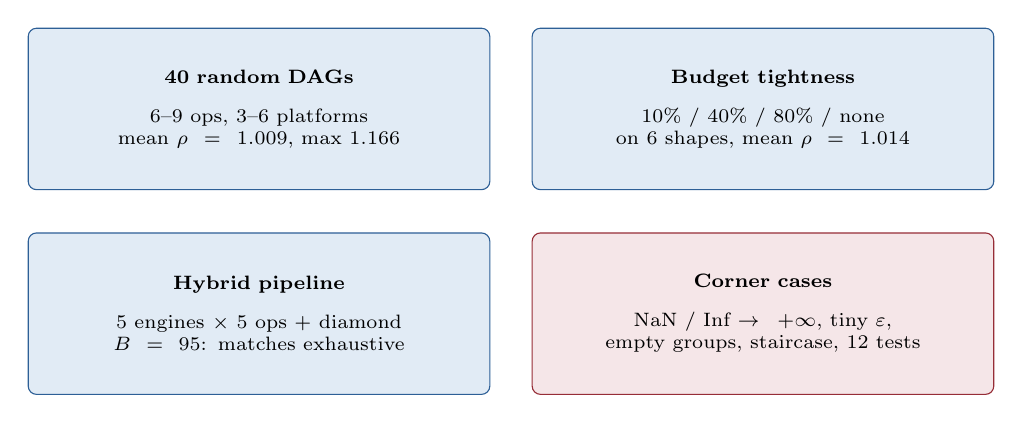
\begin{tikzpicture}[font=\small]
\node[box, text width=5.3cm, minimum height=2.05cm, inner sep=8pt] at (-3.2,1.15)
    {\textbf{40 random DAGs}\\[6pt]
    6--9 ops, 3--6 platforms\\
    mean \(\rho=1.009\), max \(1.166\)};
\node[box, text width=5.3cm, minimum height=2.05cm, inner sep=8pt] at (3.2,1.15)
    {\textbf{Budget tightness}\\[6pt]
    10\% / 40\% / 80\% / none\\
    on 6 shapes, mean \(\rho=1.014\)};
\node[box, text width=5.3cm, minimum height=2.05cm, inner sep=8pt] at (-3.2,-1.45)
    {\textbf{Hybrid pipeline}\\[6pt]
    5 engines \(\times\) 5 ops + diamond\\
    \(B=95\): matches exhaustive};
\node[box, text width=5.3cm, minimum height=2.05cm, inner sep=8pt, fill=lightred, draw=maroon] at (3.2,-1.45)
    {\textbf{Corner cases}\\[6pt]
    NaN / Inf \(\to+\infty\), tiny \(\varepsilon\),\\
    empty groups, staircase, 12 tests};
\end{tikzpicture}
\end{frame}

% ============================================================
\begin{frame}{20. Budget sweep: different work, then the original plan}

\vspace{0.08cm}
\centering
\includegraphics[width=0.88\textwidth]{budget-sweep.png}

\vspace{0.12cm}
{\scriptsize Synthetic data. Step $B$ by 1. Original Wayang $=$ min latency with no money bound (latency $80$).}
\end{frame}

% ============================================================
\begin{frame}{21. What was chosen at each budget}

\centering
\renewcommand{\arraystretch}{1.25}
\setlength{\tabcolsep}{7pt}
{\small
\begin{tabular}{@{}cllcc@{}}
\toprule
$B$ & plan & & latency & same as original? \\
\midrule
$0$--$54$ & all Java & & $280$ & no \\
$55$--$60$ & Java, then Postgres agg/sink & & $265$ & no \\
$61$--$68$ & join on Postgres & & $195$ & no \\
$69$--$93$ & Java scan, Spark join, Java rest & & $132$ & no \\
$94$--$97$ & Spark join, Postgres tail & & $111$ & no \\
$\mathbf{\ge 98}$ & \textbf{Java--Java--Spark--Spark--Java} & & $\mathbf{80}$ & \textbf{yes} \\
\bottomrule
\end{tabular}}

\vspace{0.45cm}
\begin{columns}[T]
\column{0.46\textwidth}
{\small Tight $B$: cheaper, slower work.\\
Six distinct plans as $B$ grows.}
\column{0.46\textwidth}
{\small Unbounded $B$: latency $80$, same hybrid as original min-latency Wayang.\\
$\varepsilon=0$ and $\varepsilon=0.1$ agreed on every step.}
\end{columns}
\end{frame}

% ============================================================
\begin{frame}{22. Safe pruning: four properties}

Drop a partial plan only if another can replace it for every suffix still to come.

\vspace{0.35cm}
\begin{enumerate}
\item \textbf{Same platforms already started.}\\
Startup is paid once per engine. A Java-only prefix is not the same as one that already started Spark.
\item \textbf{Same open operators.}\\
The next operator, and the conversion into it, must attach the same way. A Postgres scan is not compared with a Java scan.
\item \textbf{Better on every objective, strictly better on one.}\\
Faster-but-dearer and slower-but-cheaper both stay. Only a plan that loses on both axes is dropped.
\item \textbf{Each cost is a sum that only grows.}\\
The same suffix added to both plans keeps that order.
\end{enumerate}

\vspace{0.25cm}
{\small If 1 or 2 fails, the plans are not compared.}
\end{frame}

% ============================================================
\begin{frame}{23. Where this stops being safe}

\begin{itemize}
\item \(\varepsilon = 0.1\): a plan that is only slightly worse can be dropped.
\item Parallel branches: if latency is the \textbf{max} of the branches, not the sum, the wrong prefix can be deleted.
\item Channel conversion: one path is chosen by a single number before the front is built. The other paths are never compared.
\end{itemize}
\end{frame}

% ============================================================
\begin{frame}{24. Test bed: three checks}

{\small The scale-factor 1 run only checked answers. Monetary weight was 0, so both optimizers still picked the fastest plan.}

\vspace{0.3cm}
\begin{enumerate}
\item \textbf{Search.} Exact Pareto matches brute force on small graphs. \(\varepsilon=0.1\) is compared with exact Pareto on larger ones. Chains are easy. Diamonds, bushy joins, and fan-in are the test.
\item \textbf{Real plans, with a budget.} TPC-H scale factor 1. Q1 is the control (one scan). Q3 is the join (Pareto took 23\,s, original 8\,s). Sweep \(B\) and record the platforms chosen.
\item \textbf{Run the plan.} Put actual runtime next to the estimate. Java and Spark on this laptop show a tighter budget picks a different hybrid. Postgres is the cross-engine case, and this run did not use it.
\end{enumerate}

\vspace{0.2cm}
{\small Leave energy out until it is a third number. Report \(\rho\), subplans, enumeration time, and any budget miss.}
\end{frame}

% ============================================================
\begin{frame}{25. The paper table}

\centering
{\small Q1 and Q3. Original Wayang, exact Pareto, and \(\varepsilon=0.1\). Three budgets.}

\vspace{0.35cm}
\renewcommand{\arraystretch}{1.2}
\setlength{\tabcolsep}{5pt}
{\scriptsize
\begin{tabular}{@{}lcccccc@{}}
\toprule
& platforms & est.\ latency & est.\ money & enum.\ time & runtime & answer \\
\midrule
Q1, original & & & & & & \\
Q1, \(\varepsilon=0\) & & & & & & \\
Q1, \(\varepsilon=0.1\) & & & & & & \\
Q3, original & & & & & & \\
Q3, \(\varepsilon=0\) & & & & & & \\
Q3, \(\varepsilon=0.1\) & & & & & & \\
\bottomrule
\end{tabular}}

\vspace{0.4cm}
{\small One row per budget. Q1 answers already match the published scale-factor 1 counts. Q3 must match across the three optimizers.}
\end{frame}

% ============================================================
\begin{frame}{26. Channel conversion}

{\small The operators are already chosen. The graph only picks how the rows cross the border.}

\vspace{0.45cm}
\centering
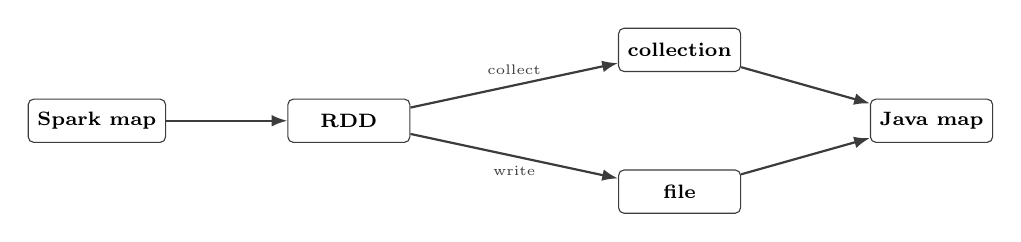
\begin{tikzpicture}[font=\scriptsize]
  \node[op] (sp) at (0,0) {Spark map};
  \node[op] (rdd) at (3.2,0) {RDD};
  \node[op] (col) at (7.4,0.9) {collection};
  \node[op] (file) at (7.4,-0.9) {file};
  \node[op] (jv) at (10.6,0) {Java map};
  \draw[arr] (sp) -- (rdd);
  \draw[arr] (rdd) -- node[above, font=\tiny] {collect} (col);
  \draw[arr] (rdd) -- node[below, font=\tiny] {write} (file);
  \draw[arr] (col) -- (jv);
  \draw[arr] (file) -- (jv);
\end{tikzpicture}

\vspace{0.4cm}
{\small Spark writes an RDD. Java reads a collection or a file. Both routes connect the same two operators.}
\end{frame}

% ============================================================
\begin{frame}{27. Two routes, one border}

\centering
\renewcommand{\arraystretch}{1.25}
\setlength{\tabcolsep}{10pt}
{\small
\begin{tabular}{@{}lcc@{}}
\toprule
route & latency & money \\
\midrule
collect the RDD & 10 & 50 \\
write a file, then read it & 40 & 20 \\
\bottomrule
\end{tabular}}

\vspace{0.55cm}
{\small Collect is faster and costs more, because it runs at the Spark rate.\\
The file is slower and cheaper.}
\end{frame}

% ============================================================
\begin{frame}{28. We keep only the cheapest route}

{\small The graph compares money only and stores the file route. The collect route is dropped before pruning, so it cannot come back.}

\vspace{0.4cm}
\begin{block}{Keeping both}
Every partial plan at that border would be copied once per route, and the next border would copy them again. Q3 is already slower for this reason (23\,s against 8\,s).
\end{block}

\vspace{0.35cm}
{\small Later work: return both routes when they trade off, and let the plan front choose.}
\end{frame}

% ============================================================
\begin{frame}{A1. From rows to milliseconds}

{\small Appendix. A load profile is how much work an operator does, not how long it takes and not the money.}

\vspace{0.5cm}
\centering
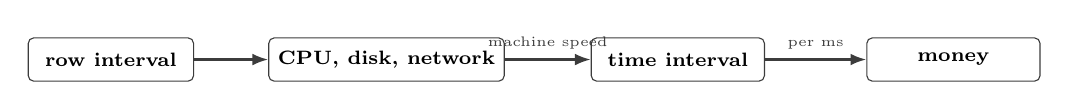
\begin{tikzpicture}[font=\scriptsize]
  \node[op, minimum width=2.1cm] (rows) at (0,0) {row interval};
  \node[op, minimum width=2.4cm] (load) at (3.5,0) {CPU, disk, network};
  \node[op, minimum width=2.2cm] (time) at (7.2,0) {time interval};
  \node[op, minimum width=2.2cm] (money) at (10.7,0) {money};
  \draw[arr] (rows) -- (load);
  \draw[arr] (load) -- node[above, font=\tiny] {machine speed} (time);
  \draw[arr] (time) -- node[above, font=\tiny] {per ms} (money);
\end{tikzpicture}

\vspace{0.45cm}
{\small The operator formula turns rows into cycles and bytes.\\
Only the last arrow uses \texttt{costs.per-ms}.}
\end{frame}

% ============================================================
\begin{frame}{A2. How the time is computed}

{\small Each resource is a straight line. Java defaults: 1 core, 2700\,MHz, 2.7\,ms per MB of disk, no network.}

\vspace{0.4cm}
\centering
\renewcommand{\arraystretch}{1.3}
\setlength{\tabcolsep}{8pt}
{\small
\begin{tabular}{@{}lll@{}}
\toprule
resource & time & Java default \\
\midrule
CPU & cycles / (cores $\times$ MHz $\times$ 1000) & $10^6$ cycles $\approx$ 0.37\,ms \\
disk & bytes $\times$ ms-per-MB / $10^6$ & 2.7\,ms per MB \\
network & bytes $\times$ ms-per-MB / $10^6$ & 0 \\
\bottomrule
\end{tabular}}

\vspace{0.4cm}
{\small The three intervals are added. Lower with lower, upper with upper.\\
Spark is the same, except network is not zero.}
\end{frame}

% ============================================================
\begin{frame}{A3. Why the result is an interval}

{\small A map formula of 100 cycles per row, on 800--1{,}200 rows, is 80{,}000--120{,}000 cycles. Both ends go through the same lines.}

\vspace{0.35cm}
\begin{columns}[T]
\column{0.48\textwidth}
\begin{block}{Then adjust}
Divide by how busy the machine is.\\
Add a fixed overhead to both ends.\\
Add the user function's own time.
\end{block}
\column{0.48\textwidth}
\begin{block}{Then price it}
Multiply both ends by \texttt{costs.per-ms}.\\
Rate 1: money is the time.\\
Spark at 5: the same milliseconds cost five times as much.
\end{block}
\end{columns}

\vspace{0.3cm}
{\small A conversion uses this same path. Collect and file-write are just small operators with their own formulas.}
\end{frame}

\end{document}
